As of the current moment the forecast component diagram for the system is as follows:

\begin{center}
    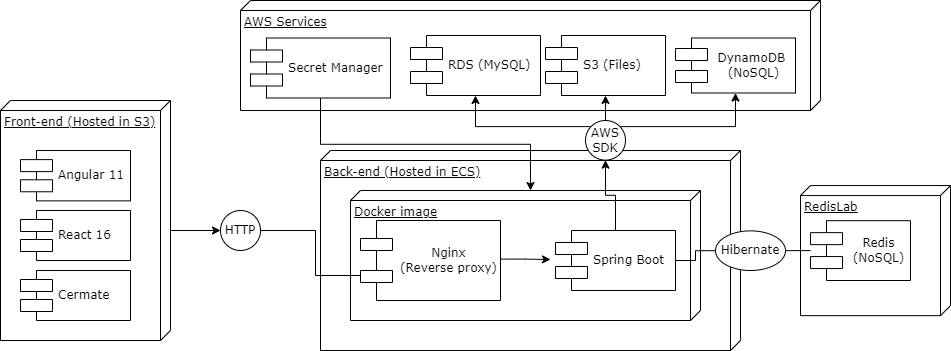
\includegraphics[width=0.8\textwidth]{images/forecast}
\end{center}

As it shows there are additional databases mainly ones for archiving files as is the case of
S3 and also archiving data for statistics down the line thus using DynamoDB\@.
Also containerizing the backend for the goal of having it run different instances seamlessly,
and have the run times duplicate efficiently.
For the creation of the images, it should be noted that they will be generated automatically,
and upload to ECR directly through CircleCI pipelines.
Thus the process of having to update or fix bugs within the back-end will be more streamlined
in a fashion that causes little to no downtime.
